\section{Hochmolekulare Stoffe - Polymere}
Hochmolekulare Stoffe bestehen aus sehr langen Molekülen, sog. \emph{Makromolekülen}, mit einer Molaren Masse von >10'000 g/mol. Makromoleküle lassen sich in kleine, sich wiederholende Abschnitte, \emph{Monomere}, unterteilen. \\

\subsection{Unterscheidung}
\begin{itemize}
	\item natürlich vorkommende hochmolekulare Stoffe, z.B. Baumwolle
	\item künstlich hergestellte hochmolekulare Stoffe (Kunststoffe)
		\begin{itemize}
			\item Thermoplaste (lineare oder verzweigte Makromoleküle)
			\item Duroplaste (engmaschig vernetzte Makromoleküle)
			\item Elastomere (weitmaschig vernetzte Makromoleküle)
		\end{itemize}
\end{itemize}

\begin{figure}[htbp]
	\centering
	\begin{subfigure}{0.25\linewidth}
		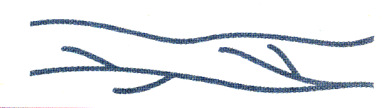
\includegraphics[width=0.9\linewidth]{images/7_Thermoplast}
		\caption{Thermoplast}
	\end{subfigure}
	\quad
	\begin{subfigure}{0.25\linewidth}
		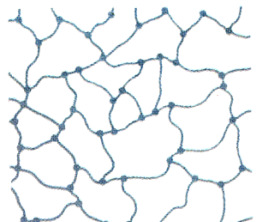
\includegraphics[width=0.9\linewidth]{images/7_Duroplast}
		\caption{Duroplast}
	\end{subfigure}
	\quad
	\begin{subfigure}{0.25\linewidth}
		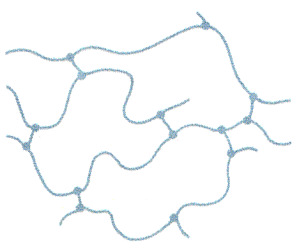
\includegraphics[width=0.9\linewidth]{images/7_Elastomer}
		\caption{Elastomer}
	\end{subfigure}
\end{figure}

\subsection{Eigenschaften}
\begin{itemize}
	\item geringe Dichte (0.8 bis 2 g/cm$^3$), weil Atome (v.a. C,H) geringe Masse haben.
	\item grosse chemische Beständigkeit, weil keine reaktionsfreudigen Gruppen.
	\item kein Siedepunkt, sondern Zersetzung, weil VdW-Kräfte oder Vernetzung
	\item sehr geringe elektrische und Wärme-Leitfähigkeit, weil keine geladenen, frei beweglichen Teilchen vorhanden
\end{itemize}

\subsection{Thermoplaste}
Bsp. Polyethen (PE), Polypropen (PP), Polyvinylchlorid (PVC), ... \\

Lineare oder verzweigte Makromoleküle. Länge: $0.001$ bis $1 \mu m$. Kettenlänge kann innerhalb des Polymers variieren. \\

Polymerisationsgrad: durchschnittliche Anzahl Monomere pro Makromolekül. \\

Thermoplaste sind teilkristallin, d.h. es können kristalline und amorphe Bereiche vorkommen.

\subsubsection{Taktizität}
Taktizität bezeichnet die räumliche Anordnung der Seitenketten / Fremdatome. Kann durch Herstellung beeinflusst werden.

\begin{figure}[htbp]
	\centering
	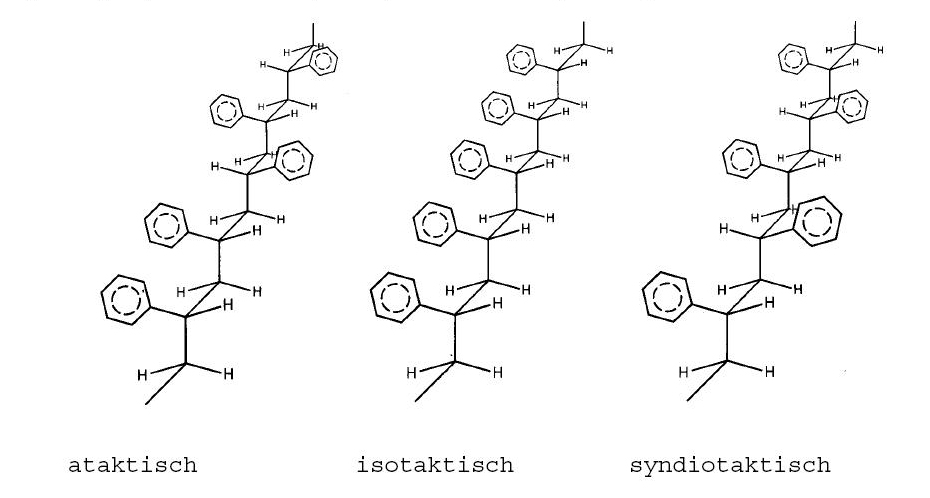
\includegraphics[width=0.7\linewidth]{images/7_Taktizitaet.png}
\end{figure}

\begin{itemize}
	\item ataktisch: amorphe Kunststoffe
	\item isotaktisch: hoher Kristallinitätsgrad möglich
\end{itemize}

\subsubsection{Eigenschaften}
\begin{itemize}
	\item schlecht löslich oder unlöslich (VdW-Kräfte)
	\item keinen Schmelzpunkt, sondern einen Schmelz\emph{bereich} (unterschiedlich starke VdW-Kräfte innerhalb)
	\item Durchlaufen beim Erwärmen versch. Aggregatzustände: fest $\rightarrow$ elastisch $\rightarrow$ plastisch $\rightarrow$ flüssig $\rightarrow$ Zersetzung
	\item Kristallinität beeinflusst Eigenschaften stark. Je kristalliner, desto höhere VdW-Kräfte
	\item Lange, unverzweigte Makromoleküle $\Rightarrow$ hohe Kristallinität, hohe Steifigkeit, hoher Schmelzbereich
\end{itemize}


\subsection{Duroplaste}
Bsp. Phenoplaste PF (Isoliermaterial, Steckdosen), Aminoplaste (Spannplattenleim), Ungesättigte Polyesterharze UP, Epoxidharze EP \\

Engmaschig vernetzte Makromoleküle $\Rightarrow$ hart, spröde, zerbrechlich, hitzebeständig (Netzstruktur bleibt beim Erwärmen erhalten) bis zur Zersetzung.

\subsection{Elastomere}
Bsp. Vernetze Polyurethane (PUR), Naturkautschuk (NR), Chloropren-Kautschuk (CR), Silikon-Kautschuk \\

Räumlich weitmaschig verknüpfte Makromoleküle $\Rightarrow$ elastisch, Zersetzung bei starkem Erwärmen.

\subsection{Herstellung von Polymeren}
Polymerisation: Verknüpfung der Monomere unter Spaltung einer Doppelbindung und Bildung einer neuen Einfachbindung $\Rightarrow$ kettenartige Makromoleküle $\Rightarrow$ Thermoplaste \\

Vulkanisation: Vernetzung von Makromolekülen mit Doppelbindungen. Ablauf: Zugabe von Schwefel $S_8$, Spaltung der $S_8$-Moleküle, Vernetzung der Makromoleküle, Produkt wird elastisch. 

\subsection{Verarbeitung von Polymeren}
Extrusion: Polymer-Granulat wird verflüssigt und mittels Druck in eine Form gepresst, z.B. Rohre, Schläuche. \\

Spritzgiessen: Wie Extrusion, jedoch wird das Polymer in eine fertige Form gespritzt, z.B. Tupperware, Kübel. \\

Blasformen: Rohling wird unter Druck und Temperatur innerhalb einer Form aufgeblasen, z.B. Getränkeflaschen. \\